%=====================================================================
\section{Model Selection and Validation}
%=====================================================================

\begin{frame}
	\frametitle{Two Questions}
	
	\begin{itemize}
		\item ``How good is our model?''
		\item ``Which model to choose among alternatives?''
	\end{itemize}
	
	\vfill
	
	\begin{columns}[onlytextwidth]
		\column{0.45\textwidth}
		\begin{block}{Problem and solution}
			\begin{itemize}
				\item ``In-sample'' performance is biased
				\item Overfitting should not be rewarded
				\item Use data splitting to get fair results
			\end{itemize}
		\end{block}
		
		\column{0.55\textwidth}
		\begin{alertblock}{Notation}
			\begin{itemize}
				\item Total loss $Q(f, D) = \sum_{(y_i, \bx_i) \in D} L(y_i, f(\bx_i))$
				\item Average loss $\bar Q(f, D) = Q(f, D) / |D|$
				\item Performance measure or evaluation metric $S(f, D)$ of interest, often $S = \bar Q$ or a function of it
			\end{itemize}
		\end{alertblock}
	\end{columns}
\end{frame}

\begin{frame}
	\frametitle{Outline}
	\begin{itemize}
		\item Nearest-Neighbor
		\item Simple Validation 
		\item Cross-Validation
		\item Test Data and Final Workflow
		\item Excursion: SQL and Spark
	\end{itemize}
\end{frame}

%=====================================================================
\subsection{Nearest-Neighbor}
%=====================================================================

\begin{frame}
	\frametitle{Excursion: $k$-Nearest-Neighbor ($k$-NN)}
	\begin{itemize}
		\item Alternative to linear model
		\item How does it work?
		\item Classification and regression
		\item Standardization?
	\end{itemize}
	
	\vfill
	
	\begin{example}
	\end{example}
\end{frame}

%=====================================================================
\subsection{Simple Validation}
%=====================================================================

\begin{frame}
	\frametitle{Simple Validation}
	\begin{itemize}
		\item In-sample, 1-NN would win any comparison!?
		\item Split data into training and validation sets $D_\text{train}$ and $D_\text{valid}$, e.g., 80\%/20\%
		\item Use performance $S(\hat f, D_\text{valid})$ on validation set to make decisions 
		
		(choose models, choose parameters like $k$)
		\item Measure amount of overfitting/optimism by 
		$$
		S(\hat f, D_\text{valid}) - S(\hat f, D_\text{train})
		$$
	\end{itemize}
	
	\vfill
	
	\begin{example}
	\end{example}
\end{frame}

%=====================================================================
\subsection{Cross-Validation}
%=====================================================================

\begin{frame}
	\frametitle{$K$-fold Cross-Validation (CV)}
	Simple validation is neither economic nor robust, except for large data
	
	\vfill
	
	\begin{columns}[onlytextwidth]
		\column{0.65\textwidth}
		\begin{block}{Algorithm}
			\begin{enumerate}
				\item Split the data into $K$ pieces $D = \{D_1, \dots, D_K\}$ called ``folds''. Typical values for $K$?
				\item Set aside one of the pieces ($D_k$) for validation
				\item Fit model $\hat f_k$ on $D \setminus D_k$
				\item Calculate performance $\hat S_k = S(\hat f_k, D_k)$
				\item Repeat Steps $2-4$ for each $k$
				\item Calculate \alert{CV performance} $\hat S_{CV} = \frac{1}{K} \sum_{k = 1}^K \hat S_k$
			\end{enumerate}
		\end{block}
		
		\column{0.35\textwidth}
		\begin{alertblock}{Remarks}
			\begin{itemize}
				\item How to choose and fit best/final model? 
				\item What means «best»?
				\item Stability of results?
				\item Repeated CV?
			\end{itemize}
		\end{alertblock}
		
		\begin{example}
		\end{example}
	\end{columns}
\end{frame}

\begin{frame}
	\frametitle{Hyperparameter Tuning}
	\begin{itemize}
		\item Choosing $k$ in $k$-NN is example of \alert{``hyperparameter tuning''}
		\item Algorithms with more than 1 hyperparameter?
		\item Grid Search CV
		\item Randomized Search CV
	\end{itemize}
\end{frame}

%=====================================================================
\subsection{Test Data and Final Workflow}
%=====================================================================

\begin{frame}
	\frametitle{Test Data and Final Workflow}
	\begin{block}{Problematic consequence of model tuning?}
		\begin{itemize}
			\item \alert{Overfitting} on validation data or on CV!
			\item Performance of final model? $\rightarrow$ \alert{Test data}
		\end{itemize}
	\end{block}
	
	\begin{columns}[onlytextwidth]
		\column{0.55\textwidth}
		\begin{block}{Workflow A}
			\begin{footnotesize}
				\begin{enumerate}
					\item Split data into train/valid/test, 
					
					e.g., by ratios 60\%/20\%/20\%
					\item Train different models on training data and assess performance on validation data. Choose best model, re-train on training + validation data, and call it ``final model'' (Simplification?)
					\item Assess performance of final model on test data
				\end{enumerate}
			\end{footnotesize}
		\end{block}
		
		\column{0.45\textwidth}
		\begin{block}{Workflow B}
			\begin{footnotesize}
				\begin{enumerate}
					\item Split data into train/test, 
					
					e.g., by ratios 80\%/20\%.
					\item Evaluate and tune different models by $K$-fold CV on training data. Choose best model, re-train on full training data
					\item Assess performance of final model on test data
				\end{enumerate}
			\end{footnotesize}
		\end{block}
	\end{columns}
	
	\begin{columns}
		\column{0.5\textwidth}
		\begin{exampleblock}{Example of Workflow B}
		\end{exampleblock}
		
		\column{0.5\textwidth}
		\alert{When test data not necessary?}
	\end{columns}
\end{frame}

\begin{frame}
	\frametitle{Ridge Regression}
	\begin{itemize}
		\item Example of \alert{penalized} regression
		\item Model equation similar to usual linear regression
		$$
		\mathbb E(Y \mid \bx) = f(\bx) = \beta_0 + \beta_1 x^{(1)} + \dots + \beta_p x^{(p)}
		$$
		\item But with penalized least-squares objective
		$$
		Q(f, D_{\text{train}}) = \sum_{(y_i, \bx_i) \in D_\text{train}} (y_i - f(\bx_i))^2 + \lambda \sum_{j = 1}^p  \beta_j^2
		$$
		\item $L2$ penalty pulls coefficients slightly towards 0, fighting overfitting
		\item $\lambda_\text{opt} \ge 0$ with best (cross-)validation result $\rightarrow$ use to fit final model
		\item Intercept? Standardization? L1? Elastic-net?
	\end{itemize}
	
	\vfill
	
	\begin{example}
	\end{example}
\end{frame}

\begin{frame}
	\frametitle{Using Independent Partitions is Essential}
	\begin{figure}
		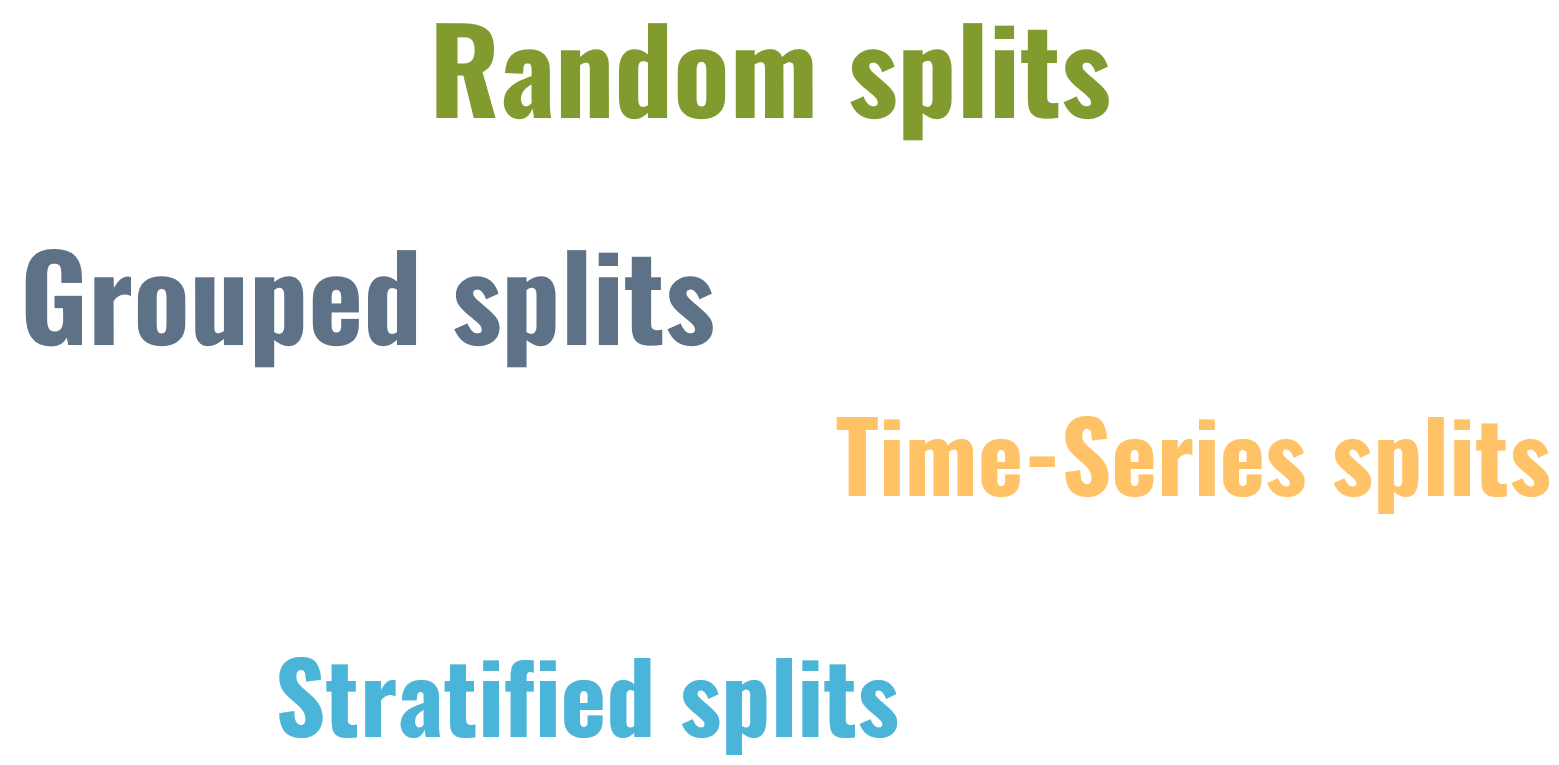
\includegraphics[width=0.8\textwidth]{pics/validation_independent.png}
	\end{figure}
\end{frame}

%=====================================================================
\subsection{Excursion: SQL and Spark}
%=====================================================================

\begin{frame}
	\frametitle{Excursion: SQL and Spark}
	\begin{quotation}
		Data science is 80\% preparing data, 20\% complaining about preparing data.
	\end{quotation}
	
	\vfill
	
	\begin{columns}[onlytextwidth]
		\column{0.5\textwidth}
		\begin{block}{Typical preprocessing steps?}
		\end{block}
		
		\begin{block}{Good moment to learn}
			\begin{itemize}
				\item data structure
				\item meaning of columns
				\item sources of bias
			\end{itemize}
		\end{block}
		
		\column{0.5\textwidth}
		\begin{block}{How to do preprocessing?}
			Data = files on disk or tables in database
			\begin{itemize}
				\item If small $\rightarrow$ R/Python
				\item If large? $\rightarrow$ Database Management System (DBMS) or Spark
				\item Communication via SQL
			\end{itemize}
		\end{block}
	\end{columns}
\end{frame}

\begin{frame}
	\frametitle{SQL}
	\begin{columns}[onlytextwidth]
		\column{0.5\textwidth}
		\begin{block}{Structured Query Language}
			\begin{itemize}
				\item Pronounced?
				\item Important in data science
				\item In DBMS or R/Python
				\item ISO norm $\leftrightarrow$ dialects
				\item SQL queries
			\end{itemize}
		\end{block}
		
		\column{0.5\textwidth}
		\begin{block}{DuckDB (since 2018)}
			\begin{itemize}
				\item In-process, open-source DBMS
				\item Easy to install in R/Python
				\item No dependencies (Java etc.)
				\item Fast
				\item Out-of-core capabilities
			\end{itemize}
		\end{block}
	\end{columns}
	
	\vfill
	
	\begin{exampleblock}{Learn SQL with examples}
		\begin{itemize}
			\item Diamonds (from memory)
			\item Taxi (from Parquet)
		\end{itemize}
	\end{exampleblock}
\end{frame}

\begin{frame}
	\frametitle{Apache Spark}
	\begin{columns}
		\column{0.5\textwidth}
		\begin{itemize}
			\item Distributed, open-source cluster computing system for big data
			\item Apache project since 2013
			\item Heavily used in industry
			\item Written in Scala
			\item Contains SQL engine
			\item Can be used from R/Python
		\end{itemize}
		
		\vfill
		
		\column{0.5\textwidth}
		
		\begin{exampleblock}{Examples}
			\begin{itemize}
				\item Diamonds (from memory)
				\item Taxi (from Parquet)
			\end{itemize}
		\end{exampleblock}
	\end{columns}
\end{frame}
